% !Mode:: "TeX:UTF-8"

\BiChapter{绪~~~~论}{Introduction}

\BiSection{课题背景及研究的目的和意义}{Background, aims and significance}
在未来的第五代移动通信(~the 5th Generation Communication Technology,5G~)网络中,
将会涌现出大量的智能移动终端,对网络的容量要求大大增加\citeup{QosUDN}。
相比于第四代移动通信(~the 4th Generation Communication Technology,4G~),
5G网络的容量需求将有1000倍的增长,
届时,终端无处不在,并且在大型的热点区域,如商场,露天展台等存在着大量的设备。
同时,不同的移动终端也会有不同的业务需求,这也就导致了业务需求的多样化。
基站的密集部署迫在眉睫。
超密集组网(~Ultra Dense Networks,UDNs~)应运而生。
超密集组网将用于满足区域面积内超高的容量需求,
为移动终端提供无缝的网络切换,让用户在无论何时,无论何地都能拥有超高速的上网和通话体验。
超密集组网在区域面积内放置了更多的基站,这是能够提供巨大容量增益一种十分可靠的技术\citeup{4LRA}。
通过在宏基站的热点区域放置微基站(~Small Base Station,SBS~)形成微小区(~Small Cell~)
提供了更高的频谱自由度,有效的提高了系统的单位面积谱效率,从而提升了系统的性能。

对宏小区(~Macro Cell~)中的宏基站(~Macro Base Station,MBS~)的部署多采用固定的格形部署,
虽然微小区也可以采用固定的格形部署,
但微小区网络的部署受到地形地貌的影响,
比如,有的地方地貌平坦,遮挡较少,适宜部署基站,有些地方地形崎岖,遮挡明显,不适宜部署基站。
微小区和异构网络的部署也受到当地人流的影响,有的地方客流量大,对容量的需求也就更加的高,因此该区域就需要密集的部署。
不仅如此,微小区网络的部署也呈现自组织性。
种种原因导致了对微小区网络的建模不能单单采用传统的基于格点的基站部署方式\citeup{ATractable}。
同时由于用户在小区中的不同位置的概率不同,比如在某些热点区域,如展会中心区,景观区,用户分布较多,
呈现从中间向四周蔓延的趋势,而在其他区域,用户不会有明显的集聚效应。


超密集在带来好处的同时,也带来了新的挑战,密集的网络使得基站之间的距离更近,
随之带来的小基站之间干扰(~Inter Cell Inference~)问题越发明显。
不仅如此,网络的密集化也导致了小区中的干扰管理算法变得越发复杂。
密集的组网也导致了很高的能耗\citeup{OFDMRA},SBS~能提供的功率也不会像宏基站提供的功率那么强,
有一定的约束,如何将有限的功率很好的利用,服务的用户更多,提供的容量更大,基站的耗能却更小,
也是现在亟需解决的热点问题。
因此需要有新的干扰管理技术,
充分协调现有的或者将要部署的~SBS~之间的关系,从而消除小基站之间的干扰,
提升用户服务质量(~Quality of Service,QoS~)提升网络的单位面积频谱利用率,达到容量提升的目的。


本课题来源于国家自然科学基金,项目名称《超密集组网中区域频谱效率理论上界及干扰管理算法研究》(项目号:61671186)。

\BiSection{国内外研究现状及分析}{Background, aims and significance}

\BiSubsection{超密集组网的研究现状}{UDNs}
2009年,业界首次提出了第五代移动通信技术(5th Generation Communication Technology,5G~)的概念。
在继承和发扬第四代移动通信技术(~4th Generation Communication Technology,4G~)的基础之上,
5G~系统的目标是提升几十被的频谱效率,百倍左右的能量效率\citeup{zhanghong},同时为了便于推广,5G~系统也需要在成本上做出考虑。
5G中的关键技术,超密集组网(~Ultra Dense Networks,UDNs~)技术,
是目前业界各个知名厂家争相研究的热点。
网络的密集化已经成为了当下移动无线组网的一个大趋势。

由于超密集组网相比宏小区网络更加复杂,网络中~SBS~的部署更加的灵活,随机,因此需要对该场景进行合理有效的建模并进行分析。
5G中的超密集组网,由于网络的拓扑结构复杂,呈现异构化,随机化,多层次,因此,不能按照传统的移动蜂窝网络,将基站建模成六边形格点的拓扑结构。
网络的建模要呈现随机性。文献\cite{ATractable}最早提出了能够体现随机化的无线多基站网络模型。
该篇文章考虑到由于网络的密集程度的提升,受到地理位置,区域对网络的需求等等随机化的影响,因此网络中基站的部署呈现随机性。
为了反应这种随机性,基于随机几何\citeup{Stogeo},提出了将基站的分布服从泊松点过程,而用户在区域内随机分布的网络拓扑模型。
并得到一种简单可行的方法,求解该场景下的中断概率、区域面积谱效率等性能。
但该篇文章只考虑了单小区单层单天线多基站,用户数量远远大于基站数量的情况,
且没有对用户的统计特性进行分析\citeup{4LRA}。
文献\cite{2LayerPC}提出了单小区双层多基站超密集无线网络模型,并分析了该场景下的能耗特性。
文献\cite{UDNMIMO}在前两篇文章的基础上,提出了单小区多层异构的网络,小区中的基站配备多根天线,
该文献还考虑了基站数量和用户数量的关系,并重点分析了基站和用户数量相当的情况下网络的性能。
并给出了在该场景下的基站睡眠和唤醒机制的算法。给出了能达到最大单位面积谱效率下,小区内部署基站的密度。
文献\cite{user-centric}提出了以用户为中心的超密集组网的网络模型。该模型假设小区中的基站服从泊松点过程,小区中的用户随机分布,
小区中的用户的数量与基站的数量相当,或者小于基站的数量。该模型假设网络采用了干扰协调算法,
并假设距离用户最近的基站为用户进行服务,并设定一个距离门限,将距用户距离不超过距离门限的基站作为干扰协调基站,
用于协调其他用户和基站所建立的链路对该用户的影响。

在超密集组网场景下,由于系统中的用户较多,容量需求大,因此,需要网络能够提供更高的单位面积的频谱利用率\citeup{datamaxudn}。
同时,通信已经成为世界上最耗能的应用\citeup{costudn},因此要想办法在满足用户要求的同时,尽可能的降低能耗,从而得到较高的能耗比,即网络需要有很高的单位面积能量谱效率。
超密集组网(UDN)作为~5G~的关键技术之一,对其概念的描述、网络布置的探索、性能分析和具体干扰管理算法的研究,
随着对~5G~标准的不断探索,这些方面的研究将是未来的重点和热点方向。

许多热点技术也可以应用到超密集组网场景中,
如开发新的频谱资源以达到网络容量提升的毫米波(~Millimeter Wave Technology~)技术;
通过使用大规模多输入多输出系统(~Massive Multiple-Input Multiple-Output,Massive MIMO~)、
高阶调制如稀疏码多址技术(~Sparse Code Multiple Acess,SCMA~)等方式也可以在给定的频率资源上增加频谱资源的利用效率;
与此同时,在超密集组网场景下,基站之间距离较近,
基站之间的协作更便利,因此也可以使用多点联合传输(~Coordinated Multipoint,CoMP~)技术进一步提升网络的性能。

\BiSection{超密集组网的网络架构}{The construction of UDN}
超密集组网需要好的网络架构对网络的性能进行优化,对网络中的干扰进行管理。
本小节中介绍超密集组网网络架构中较有潜力的,可以被应用的具有前景的网络架构,
重点介绍云接入网络(~Cloud Radio Acess Network,C-RAN~)架构
和多用户多点联合传输(Multi-User Coordinated Multipoint,Multi-User CoMP)。

\BiSubsection{C-RAN}
C-RAN架构最大的特点是基带资源池化特性,基带资源可以在不同的基站之间共享。
基于虚拟基带处理单元池和遥控射频端的联合,相比于其他的蜂窝网络,C-RAN架构有更低的网络延时。
CRAN~网络架构如图~\ref{CRAN}~所示。
\begin{figure}[htbp]
\centering
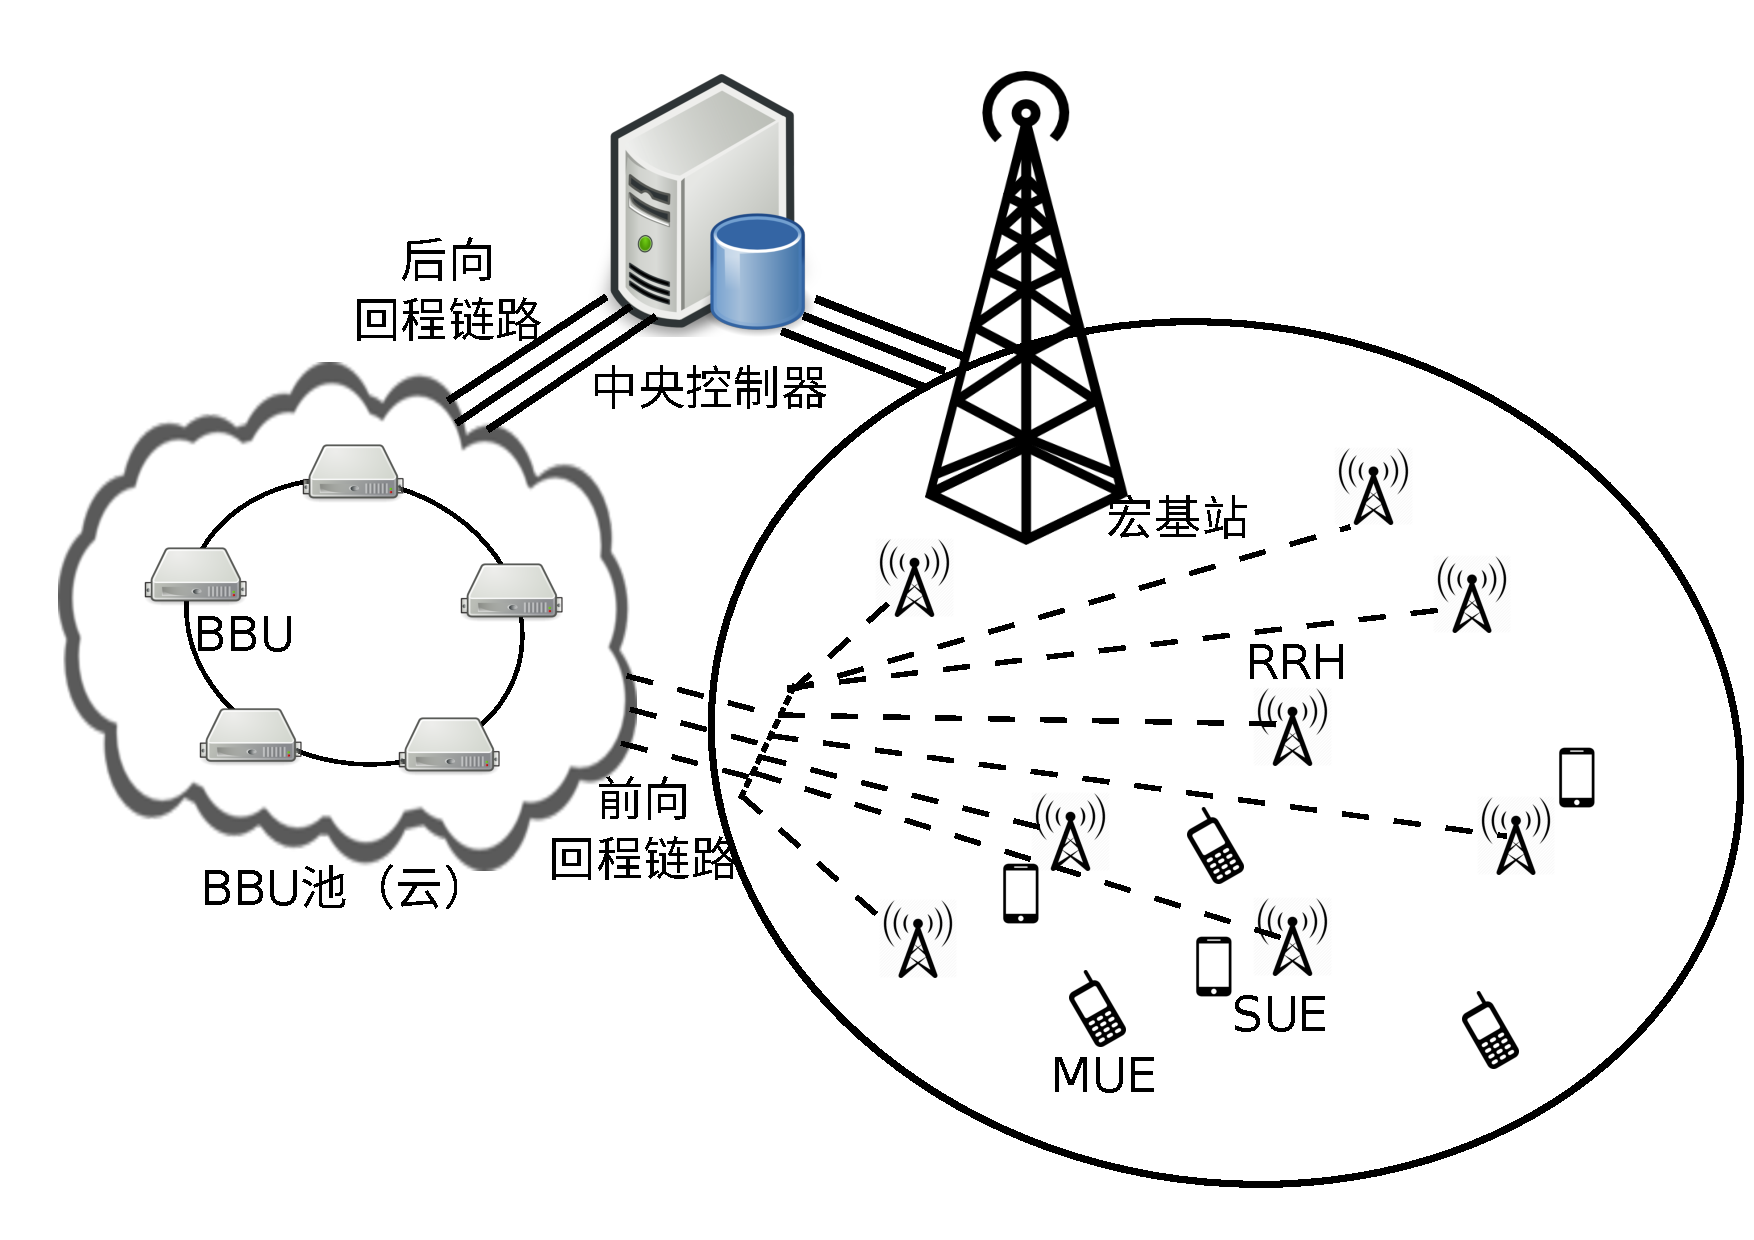
\includegraphics[width = 0.62\textwidth]{H-C-RAN_PPP.pdf}
\caption{CRAN~网络架构的示意图}\vspace{-1.5em}
\label{CRAN}
\end{figure}
从图~\ref{CRAN}~中可以看出,网络主要有三个部分组成,分别为中央控制器,基带处理单元池(~BBU~)池
遥控射频头(~RRH~),~BBU~池通过后向回程链路(~Backhaul~)与中央控制器相连接,
通过前向回程链路(~Fronthaul~)与~RRH~相连接。
再一次下行通信中,中央控制器主要完成网络层上的协议,如小区切换、跨区访问等\citeup{greencran}。
信号经过网络层的处理通过后向回程链路下发到物理层,
由~BBU~池完成基带信号的处理,其中包括小区分簇\citeup{clustercran}、多用户联合传输\citeup{compcran}、预编码\citeup{mmimocran}、调制、信道编码等\citeup{jthcran}。
经过基带处理的信号通过前向回程链路传输到~RRH,在~RRH~上完成数模转换和功率放大等射频端的过程。
上行链路的通信是下行链路的逆过程,每个部分完成的功能也大致相同。
CRAN~通过将网络层、基带处理、射频处理三者分离,将需要运算复杂度较高的基带处理部分从基站端剥离,
将多个基站的基带信号处理单元放置在云端,将最新的云计算技术应用到信号处理当中,
网络的运算能力大大增强\citeup{d2dcran2}。
除此之外,由于云端的~BBU~池与小区内的微基站~RRH~均进行了连接,
因此可以将小区内的微基站的新到状态信息汇总,使得最新的分布式的技术,如分布式~MIMO技术、
分布式预编码技术的使用成为了可能。

CRAN是干扰协调和频谱资源管理的有效的方法。由于RRH结构简单,RRH可以以较低的硬件成本进行密集的布放,BBU池化后资源统一调度,能量效率更高。
由于中心化的架构,多用户干扰可以被诸如CoMP这样的多点协作技术有效的解决掉,这样将会有很有效的性能增益。
在传统的CRAN架构中(4G),C-RAN被部署用于连接宏基站和BBU池,由于BBU和RRH之间的传输路径长,这种传统的基站会造成很大的传输时延,而在密集热点区域采用C-RAN架构,延迟也会被大大的缩短。
不仅如此,它还是有效解决潮汐效应的一种方式\citeup{interference_lim_cran}。

但CRAN架构也不是完美的。若要将CRAN架构应用于超密集组网当中,需要减小功耗\citeup{icccran},建立RRH睡眠与活跃状态的选择机制。
不仅如此,还要实现低花费的前向链路,因为前向链路能够提供的能量资源是有限的。
同时也要降低网络中算法的复杂度,降低训练开销。
联合传输技术(~CoMP~)最早有3GPP提出\citeup{jointaseeeopt},应用联合传输技术,
基站通过后向回程链路相互连接在一起\citeup{compund2},
同时为用户提供服务,在多用户联合传输系统下,基站可以采用预编码等技术为多个用户同时提供服务。

联合传输技术是伴随第四代移动通信~(4G)~提出的一个关键技术\citeup{compca}。
其主要的思想是以用户为中心,将基站联合起来,进行协作,
共同对用户进行服务\citeup{uplinkcomp}。
由于基站间相互联合共同服务区域内的用户用户,
处在基站边缘的用户的干扰功率也能被用户利用成为有用的接收功率,从而使得边缘用户的有效性大大提升\citeup{compudn3}。
联合传输的架构示意图如图~\ref{CoMP}~所示,
\begin{figure}[htbp]
\centering
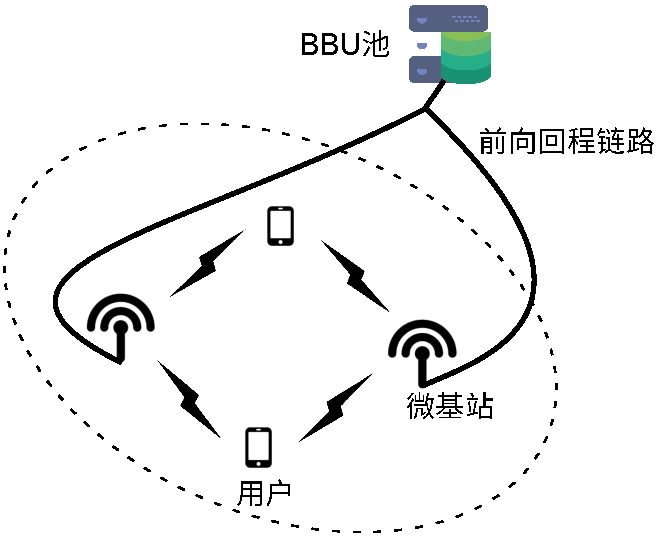
\includegraphics[width = 0.62\textwidth]{CoMP.pdf}
\caption{联合传输网络架构示意图}\vspace{-0.5em}
\label{CoMP}
\end{figure}
从图中可以看到,网络由用于处理数字信号的BBU池,用户传输信号的微基站和前向回程链路组成。
传送给用户的信息首先通过BBU池进行数据处理,在通过前向回程链路传输到基站端,由于采用了干扰消除算法,因此两个基站传送给用户的信息均为用户可以利用的有效信号,
实现两个基站联合传输共同服务区域内的用户的目的。
\BiSubsection{小区资源管理和调度算法的研究现状}{MIMO}

OFDM小区间干扰严重,与CDMA的区别,都有那些减小的技术

小区中的资源管理和调度算法,是伴随移动无线通信网络诞生开始就面临的一个难点。
由于频谱资源,时间资源,空间资源都是有限的,为了利用有限的网络资源,我们不得不采用将空间划分成为许多个小区,每个小区中放置基站对小区中的用户进行服务。
在前几代蜂窝移动通信网络中,采用频率复用技术解决小区之间的干扰问题。

蜂窝移动通信网络初期,由于网络中服务的用户量较小,网络众多用户对容量的需求较低,设备较为落后。小区之间多采用较为简单的频率复用的调度方法。
相邻的小区之间采用不同的频谱资源,每个小区所分配的频谱资源相同。这样的好处是可以几乎彻底的解决小区之间的干扰。
但是同样的,由于每个小区所分配的频谱资源相同且固定不利于针对不同小区之间容量需求的不均匀的情况,网络的自适应调节能力较差。
由于相邻的小区采用不同的频谱资源,导致小区的可用频谱资源降低一倍以上,因此虽然提升了小区内用户的统计覆盖率,但是,
去使小区的单位面积谱效率有较大的损失。而超密集组网网络场景下,网络系统需要满足大连接,高速率的需求,区域面积频谱利用率显然是一个非常重要的指标。
在静态频率复用的基础之上,出现了更加复杂的基于频率复用的小区资源管理和调度算法。

在众多频率复用算法中,软频率复用是一种可靠的频率复用技术,该技术由华为提出\citeup{yangxuezhi},并应用与4G组网的场景下。软频率复用是传统的复用技术的改进。
软频率复用技术,通过设定发射功率门限,区分不同频率的使用。这样做,使得相邻的小区不一定要使用完全不同的频率资源,而是只需要相邻小区的边缘用户使用不同的频率。
而小区中心的用户距离相邻基站的距离较远,收到相邻基站的影响较小,因此虽然使用相同的频率资源,但实际上用户与服务基站构成的通信链路并不会受到相邻基站的干扰的强烈的影响。

软频率复用的方法虽然解决了之前频率复用系统频谱利用率较低的问题,但是用于小区中的频谱资源是固定的,并没有考虑小区与小区之间的网络容量需求不均匀的问题,因此网络的动态性较差。
由于硬件性能的提升,网络机构的逐渐发展。小区与小区之间可以共享一部分信息,并且中心控制器也可以控制多个小区,因此,可以采用单个中心控制器控制多个小区,将多个小区的资源混合在一起做一个统筹。
多个小区之间进行动态的频率复用。基于该思想,文献\cite{4LRA}提出了一种多小区动态频率资源分配的算法,该算法基于图论的思想,应用贪婪算法对图中的节点进行着色,完成频率资源的分配。
但是该频率资源分配算法采用贪婪算法,不能达到性能的最优,需要进一步的引入小区中基站的分布规律和分布特点,以及用户的分布规律和特点。
引入比贪婪算法更优秀的图论优化的算法达到性能的最优。

预编码技术也是进行干扰管理和消除的一个重要的技术。
预编码最早由Tomlinson提出,用于单输入单输出(SISO)系统当中。
预编码的主要思想是由于发射机多为基站,其提供的功率很高,这就允许了基站可以做的很复杂,许多算法可以在基站端实现的话,就可以减少很多手机终端的负担。
除此之外,由于基站端知道所有用户的信道状态信息,因此,基站可以利用所得到的信道状态信息进行干扰消除。
由于不同的用户和基站构成的信道链路不相同,因此由信道状态因数构成的信道矩阵可以构成一个向量空间,
根据预编码技术,用户所发送的信息可以等效为向量空间中的一个向量,可以利用向量与向量之间的相关性来刻画不同链路之间的干扰。
预编码就是利用信道状态信息,使得多个天线之间组成的链路尽量的正交。
文献\cite{DisPrecode}发明了一种分布时预编码的预编码算法,由于超密集组网的特性,网络中的基站较为密集,这也就使得不同的基站之间可以共享部分信道状态信息。
系统可以等效为一个多输入多输出(MIMO)系统。应用预编码技术,用户之间的干扰会有显著的降低。
文献\cite{LayerPrecode}和\cite{Layer2Precode}采用分层的方法,首先进行单小区的分析,之后进行多小区的预编码,虽然采用分层次的预编码技术不能够使得性能达到最优。
但是采用层次化的设计,可以在每一层都可以达到局部的最优或次优,却显著的降低了算法的复杂度。

不仅如此,基于超密集组网场景的特性,基站的部署较为密集,因此,经常会出现用户的数量与基站的数量相当,或者用户的数量与基站的数量相比更少。
因此在5G系统中,引入了以用户为中心的联合传输策略。其主要的思想是去距离用户近信道信息较好的基站为服务基站。而其他的接收功率大于预设门限的基站作为干扰协调的基站,协调其他用户与基站之间构成的链路对该用户的干扰。
文献\cite{Ucent}提出了以用户为重新的干扰管理算法,并且引入了联合传输技术,用户的总的接收功率有了显著的提升,干扰的功率有了显著的降低。
文献\cite{CoMPUDN}提出了基于多点联合传输(CoMP)的干扰管理算法,提出以用户为中心的干扰管理算法。通过仿真,文中证明以用户为中心的干扰管理算法有效的缓解了小区间的干扰。
文献\cite{UNOMAcent}采用以用户为中心的策略,针对超密集组网网络场景,结合最新的非正交多址(NOMA)调制技术。文章通过仿真证明了系统的单位面积频谱效率有了显著的提升。

虽然小区资源管理和调度算法已经被研究多年,但由于超密集组网网络场景的提出,网络的场景越来越复杂,再加上近几年许多新的网络架构的出现。
为了解决当下稀缺的频谱资源与不断增加的用户和用户需求之间的矛盾。必须要设计出一套新的干扰管理和资源分配算法,协调小区间的干扰,增加单位面积的频谱利用率,提高网络的能量效率。


\BiSubsection{国内外研究现状简析}{Analysis}
超密集组网是5G中的重要的技术,5G要覆盖主要的三个场景,即高速率场景,大连接场景,低时延场景。
而超密集组网网络是解决在大连接的情况下,满足网络中的用户能在很高的速率之下运行。
因此研究超密集组网网络场景下的技术,在5G中有着至关重要的作用。
在当下,调制技术,编码技术等5G中关键的技术都已经基本的确定了,5G研究的中心也逐渐转移至网络层。

网络层面上,随着第五代移动通信技术的发展与推广以及计算机领域和电子硬件领域的进步,网络架构层面上,也有了很多发展。
其中CRAN技术、FRAN技术、异构网络技术、软件定义网络(SDN)技术都有潜力为超密集组网的网络架构提供网络架构层面的参考。
但是现在还没有一个已经确定的针对超密集组网网络场景下的一个很好的优化方案。
在超密集组网的网络架构中,要避免网络消耗过大,前向链路容量需求过大,计算复杂度过高,延时过高的现有网络架构的不足。
还有能够支持大连接高速率的需求。

由于网络的干扰管理算法从移动蜂窝网络发明和推广开始就一直是组网的重点问题。
但目前并没有很好的针对超密集组网网络场景的特性,进行合理优化的比较有效的算法。



\BiSection{本文研究内容及组织结构}{Content and structure}
本文首先对超密集组网中用到的基本的技术进行阐述和探究。对超密集组网网络场景中有潜力的技术进行了总结,对关键参数进行了深入的讨论。
接着,根据超密集组网网络场景的特性。
针对网络中基站和用户的统计特性,对密集热点区域无线网络的网络场景进行了建模分析,得到了理论上的网络覆盖率和单位面积频谱利用效率的边界。
最后,针对超密集组网的网络场景,网络拓扑结构,网络统计特性,基于二分图模型,提出了一种低复杂度的资源分配和干扰管理算法。
仿真证明,该资源分配和干扰管理算法复杂度较之前算法更低,并且支持的用户数和系统的和容量好于传统同复杂度的算法。
章节安排如下:

第~1~章:介绍课题背景及研究的目的和意义,叙述国内外在超密集组网和干扰管理和资源分配算法两方面的研究现状以及存在的问题,给出本文的研究内容。

第~2~章:对超密集组网网络场景中可行的网络架构和合理的系统模型进行了介绍,对关键参数进行了深入的讨论。

第~3~章:针对网络中基站和用户的统计特性,对密集热点区域无线网络的网络场景进行了建模分析,得到了理论上的网络覆盖率和单位面积频谱利用效率的边界。

第~4~章:针对密集热点区域无线网络的网络特性,对网络进行优化,首先采用分簇算法对基站进行分簇,接着对将统一簇内的基站
通过~CRAN~网络架构进行联合,对簇内采用基于~ZFBF~的多用户联合传输技术。
仿真结果证明,该干扰管理策略有效地优化了网络的覆盖率和单位面积频谱效率的性能。
